% Esquema conceptual del resample diario de O1 (capítulo 3, §3.4).
% Ilustra: hora de referencia 08:00 UTC, ventana de tolerancia +/-60 min,
% selección del fix más cercano (menor delta_minutes) y un día-hueco (NaN).
% Ilustrativo (no es figura de decisión). Compila standalone a PDF.
\documentclass[border=8pt]{standalone}
\usepackage[T1]{fontenc}
\usepackage[utf8]{inputenc}
\usepackage{lmodern}
\usepackage{tikz}
\usepackage{xcolor}
\usetikzlibrary{arrows.meta, positioning, shapes.geometric, decorations.pathreplacing}

\definecolor{azul}{HTML}{1F4E79}
\definecolor{azulcielo}{HTML}{2E86C1}
\definecolor{gris}{HTML}{777777}
\definecolor{rojo}{HTML}{C0392B}

\begin{document}
% Escala: 1 unidad x = 1 hora (desplazada: unidad = hora - 4). x=0.62cm/h.
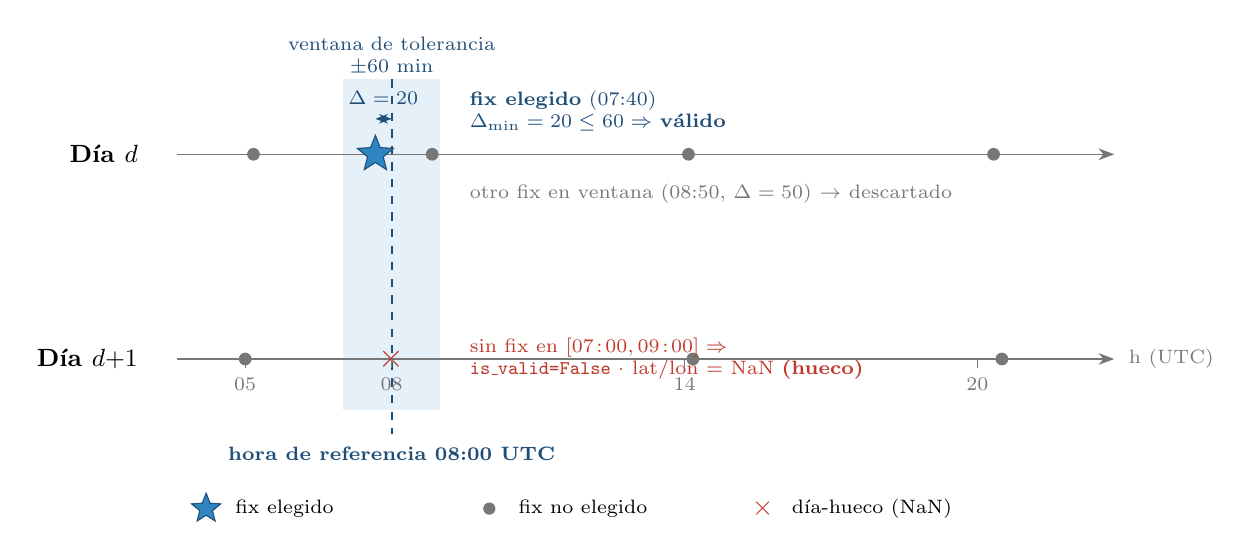
\begin{tikzpicture}[x=0.62cm, y=1cm, font=\sffamily\small]

  \def\yd{0}      % día d (con fix válido)
  \def\ydd{-2.6}  % día d+1 (hueco)

  % --- Banda de tolerancia [07:00, 09:00] detrás de todo ---
  \fill[azulcielo!12] (3,\ydd-0.65) rectangle (5,\yd+0.95);
  \node[azul, font=\scriptsize, align=center] at (4,\yd+1.25)
    {ventana de tolerancia\\$\pm 60$ min};

  % --- Línea de la hora de referencia (08:00) ---
  \draw[azul, dashed, thick] (4,\yd+0.95) -- (4,\ydd-0.95);
  \node[azul, font=\scriptsize\bfseries] at (4,\ydd-1.2) {hora de referencia 08:00 UTC};

  % ===================== DÍA d =====================
  \node[anchor=east, font=\small\bfseries] at (-1.0,\yd) {Día $d$};
  \draw[-{Stealth[length=2mm]}, gris] (-0.4,\yd) -- (18.8,\yd);

  % fixes del día d (gris = no elegido); coords en (hora-4)
  \fill[gris] (1.17,\yd) circle (2.3pt);   % 05:10
  \fill[gris] (4.83,\yd) circle (2.3pt);   % 08:50 (dentro de ventana, delta=50)
  \fill[gris] (10.08,\yd) circle (2.3pt);  % 14:05
  \fill[gris] (16.33,\yd) circle (2.3pt);  % 20:20

  % fix elegido: 07:40 (dentro de ventana, delta=20 -> menor) = estrella azul
  \node[star, star points=5, star point ratio=2.3, fill=azulcielo, draw=azul,
        inner sep=2.1pt] (chosen) at (3.667,\yd) {};

  % medida de delta_minutes (07:40 -> 08:00)
  \draw[{Stealth[length=1.6mm]}-{Stealth[length=1.6mm]}, azul, thin]
        (3.667,\yd+0.45) -- (4,\yd+0.45);
  \node[azul, font=\scriptsize] at (3.83,\yd+0.72) {$\Delta=20$};

  \node[azul, font=\scriptsize, anchor=west, align=left] at (5.4,\yd+0.55)
    {\textbf{fix elegido} (07:40)\\ $\Delta_{\min}=20\le 60 \Rightarrow$ \textbf{válido}};
  \node[gris, font=\scriptsize, anchor=west] at (5.4,\yd-0.5)
    {otro fix en ventana (08:50, $\Delta=50$) $\rightarrow$ descartado};

  % ===================== DÍA d+1 =====================
  \node[anchor=east, font=\small\bfseries] at (-1.0,\ydd) {Día $d{+}1$};
  \draw[-{Stealth[length=2mm]}, gris] (-0.4,\ydd) -- (18.8,\ydd);

  % fixes del día d+1: ninguno dentro de [07,09]
  \fill[gris] (1.0,\ydd) circle (2.3pt);    % 05:00
  \fill[gris] (10.17,\ydd) circle (2.3pt);  % 14:10
  \fill[gris] (16.5,\ydd) circle (2.3pt);   % 20:30

  % marca de hueco en la hora de referencia
  \node[rojo, font=\large\bfseries] at (4,\ydd) {$\times$};
  \node[rojo, font=\scriptsize, anchor=west, align=left] at (5.4,\ydd)
    {sin fix en $[07\!:\!00, 09\!:\!00] \Rightarrow$\\ \texttt{is\_valid=False} · lat/lon $=$ NaN \textbf{(hueco)}};

  % --- Etiquetas de horas (picos de muestreo) sobre el eje del día d+1 ---
  \foreach \h/\lbl in {1/05, 4/08, 10/14, 16/20} {
     \draw[gris] (\h,\ydd) -- (\h,\ydd-0.12);
     \node[gris, font=\scriptsize, below] at (\h,\ydd-0.12) {\lbl};
  }
  \node[gris, font=\scriptsize, anchor=west] at (18.9,\ydd) {h (UTC)};

  % --- Leyenda ---
  \begin{scope}[shift={(0,\ydd-1.9)}]
    \node[star, star points=5, star point ratio=2.3, fill=azulcielo, draw=azul,
          inner sep=1.7pt] at (0.2,0) {};
    \node[anchor=west, font=\scriptsize] at (0.6,0) {fix elegido};
    \fill[gris] (6.0,0) circle (2.2pt);
    \node[anchor=west, font=\scriptsize] at (6.4,0) {fix no elegido};
    \node[rojo, font=\bfseries] at (11.6,0) {$\times$};
    \node[anchor=west, font=\scriptsize] at (12.0,0) {día-hueco (NaN)};
  \end{scope}

\end{tikzpicture}
\end{document}
